\section{Capability Maturity Model Integration}
Nowadays companies want to deliver products and services better, faster and cheaper.
At the same time, in the high-technology environment of the twenty-first century, nearly all organizations have found themselves building increasingly complex products and services.
It's unusual today for a single organization to develop all the components that compose a complex product or service. More commonly, some components are built in-house and some are acquired; then all the components are integrated into the final product or service.
Organizations must be able to manage and control this complex development and maintenance process.
The problems these organizations address today involve enterprise-wide solutions that require an integrated approach.
Effective management of organizational assets is critical to business success. In other words, these organizations are product and service developers that need a way to manage their development activities as part of achieving their business objectives.
In the current marketplace, maturity models, standards, methodologies, and guidelines exist that can help an organization to improve the way it does business.
However, most available improvement approaches focus on a specific part of the business and do not take a systematic approach to the problems that most organizations are facing.
So, focusing on improving one particular business area, these models are hindered by barriers that exist in organizations.
\textbf{CMMI} for development (CMMI-DEV) provides an opportunity to avoid or eliminate these barriers.
It consists of best practices that address development activities applied to products and services.
It addresses practices that cover the product's lifecycle from conception through delivery and maintenance.
The goal is to build and maintain the total product.
CMMI-DEV contains 22 process areas.
Of those process areas, 16 are core process areas, 1 is a shared process area and 5 are development specific process areas.
The Software Engineering Institute (SEI) in its research, has found some key points on which organizations can focus on improving their business.
\begin{center}
      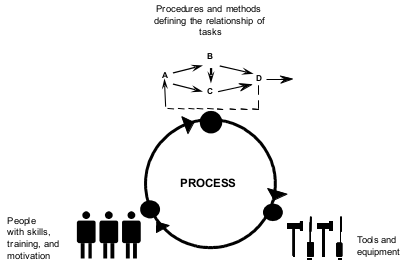
\includegraphics[scale=0.40]{images/SEI_key_points.png}
\end{center}
In particular, these key points are: people, procedures and methods, and tools and equipment.
These points are kept together by the processes used in our organization.
They allow us to address scalability and provide a way to incorporate knowledge of how to do things better.
Processes allow us to leverage our resources and to examine business trends.
We are focusing on methodologies, not because people and technologies aren't important, but since the technology changes at an incredible speed and people can works for different companies, in this way we can provide the infrastructure and stability necessary to deal with an ever-changing world and to maximize the productivity of people and the use of technology to be competitive.
The SEI has taken the process management premise "the quality of a system of a product is highly influenced by the quality of the process used to develop and maintain it" and defined CMMs that embody this premise.
A CMM, including CMMI, is a simplified representation of the world, which contains the essential elements of effective processes.
CMMs focus on improving processes in an organization, describing an evolutionary path from an immature process to a disciplined mature process with improved quality and effectiveness.
CMMI can be used in process improvements also as a framework, which provides the structure needed to produce CMMI models, training, and evaluation components.
To allow the use of multiple models withing the CMMI framework, model components are classified as either common to all CMMI models or applicable to a specific model.
The common material is called \textbf{CMMI Model Foundation} (CMF).
The components of the CMF are part of every model generated from the CMMI framework.
Those components are combined with material applicable to an area of interest to produce a model.
A \textbf{constellation} is defined as a collection of CMMI components that are used to construct models, training materials, and evaluate related documents for an area of interest. CMMI-DEV previously introduced is the development constellation for a model.
All CMMI models contain multiple \textbf{Process Areas} (PAs).
A process area is a cluster of related practices in an area that, when implemented collectively, satisfies a set of goals considered important from making improvements in that area.
Some of these areas are: Causal Analysis and Resolution (CAR), Configuration Management (CM), etc.
We can define two types of goal:
\begin{itemize}
      \item \textbf{Generic}: it's called generic because the same goal statement applies to multiple process areas. A generic goal describes the characteristics that must be present to institutionalize processes that implement a process area. It's a required model component and is used in the evaluation to determine whether a process area is satisfied or not. Institutionalization is an important concept in process improvement since it implies that the process is ingrained in the way the work is performed and there is a commitment and consistency to perform the process. The progress of process institutionalization is characterized by the type of generic goal:
            \begin{itemize}
                  \item \textbf{GG1 \- Performed process}: a performed process is a process that accomplishes the work necessary to satisfy the specific goals of a process area.
                  \item \textbf{GG2 \- Managed process}: a managed process is a performed process that is planned and executed in accordance with some policy. It employs skilled people having adequate resources to produce controlled outputs. It's controlled, monitored, reviewed, and evaluated for adherence to its process description. The process can be instantiated by a project, group, or organizational function. Management of the process is concerned with institutionalization and the achievement of other specific objectives established for the process, such as cost, schedule, and quality objectives. The control provided by a managed process helps to ensure that the established process is retained during times of stress. The requirements and objectives for the process are established by the organization. The status of the work products and services are visible to management at defined points. Commitments are established among those who perform the work and the relevant stakeholders and are revised as necessary. Work products are reviewed with relevant stakeholders and are controlled. A critical distinction between a performed process and a managed process is the extent to which the process is managed. A managed process is planned and its execution is managed against the plan. Corrective actions are taken when the actual results and execution deviate significantly from the plan. A managed process achieves the objectives of the plan and is institutionalized for consistent execution.
                  \item \textbf{GG3 \- Defined process}: a defined process is a managed process that is tailored from the organization's set of standard processes according to the organization's tailoring guidelines. It has a maintained process description and contributes process-related experiences to the organizational process assets. Organizational process assets are artifacts that relate to describing, implementing, and improving processes. These artifacts are assets because they are developed or acquired to meet the business objectives of the organization and they represent investments by the organization expected to provide current and future business value. The organization's set of standard processes, which are the basis of the defined process, are established and improved over time. Standard processes describe the fundamental process elements that are expected in the defined processes. Standard processes also describe the relationships among these process elements. A project's defined process provides a basis for planning, performing, and improving the project's task and activities. A critical distinction between a managed process and a defined process is the scope of application of the process descriptions, standards, and procedures. For a managed process, the process descriptions, standards, and procedures are applicable to a particular project, group, or organizational function. As a result, the managed processes of two projects in one organization can be different. Another critical distinction is that a defined process is described in more detail and is performed more rigorously than a managed process. Finally, management of the defined process is based on the additional insight provided by an understanding of the interrelationships of the process activities and detailed measures of the process, its work products, and its services.
            \end{itemize}
      \item \textbf{Specific}: a specific goal describes the unique characteristics that must be present to satisfy the process area. It's a required model component and is used in the evaluation to determine whether a process area is satisfied or not.
\end{itemize}

\subsection{Understanding levels}
Levels are used in CMMI-DEV to describe an evolutionary path recommended for an organization that wants to improve the processes it uses to develop products or services.
CMMI supports two improvement paths using levels.
One path enables organizations to incrementally improve processes corresponding to an individual process area selected by the organization.
The other path enables organizations to improve a set of related processes by incrementally addressing successive sets of process areas.
These two improvement paths are associated with the two types of levels: \textbf{capability levels} and \textbf{maturity levels}.
These levels correspond to two approaches to process improvement called \textbf{representations}.
In turn, the two representations are called \textbf{continuous} and \textbf{staged}.
Both representations provide ways to improve our processes to achieve business objectives and use the same model components.
The continuous representation is concerned with selecting both a particular process area to improve and the desired capability level for that process area.
The staged representation is concerned with selecting multiple process areas to improve within a maturity level.
Both capability levels and maturity levels provide a way to improve the processes of an organization and measure how well organizations can and do improve their processes.
However, the associated approach to process improvement is different.

\subsubsection{Capability levels (Continuous representation)}
To support those who use the continuous representation, all CMMI models reflect capability levels in their design and content.
The four capability levels, each of them is a layer for the process improvement, are designated by the numbers 0 through 3:
\begin{itemize}
      \item \textbf{0. Incomplete}: an incomplete process is a process that either is not performed or is partially performed. One or more of the specific goals of the process area are not satisfied and no generic goals exist for this level since there is no reason to institutionalize a partially performed process.
      \item \textbf{1. Performed}: a performed process is a process that accomplishes the needed work to produce work products; the specific goals of the process area are satisfied.
      \item \textbf{2. Managed}: a managed process is a performed process that is planned and executed in accordance with some policy; it employs skilled people having the adequate resources to produce controlled outputs; it involves relevant stakeholders; it's monitored, controlled, reviewed, and evaluated for adherence to its process description. The process discipline reflected by capability level 2 helps to ensure that existing practices are retained during times of stress.
      \item \textbf{3. Defined}: a defined process is a managed process that is tailored from the organization's set of standard processes according to the organization's tailoring guidelines and contributes work products, measures, and other process improvement information to the organizational process assets.
\end{itemize}

\subsubsection{Maturity levels (Staged representation)}
To support those who use the staged representation, all CMMI models reflect maturity levels in their design and content.
A maturity level is a defined evolutionary plateau for organizational process improvement.
Each maturity level matures an important subset of the organization's processes, preparing it to move to the next maturity level.
The maturity levels are measured by the achievement of the specific and generic goals associated with each predefined set of process areas.
The five maturity levels are designated by the numbers 1 through 5:
\begin{itemize}
      \item \textbf{1. Initial}: in this layer processes are usually ad hoc and chaotic. In spite of this chaos, maturity level-1 organizations often produce products and services that work, but they frequently exceed the budget and schedule documented in their plans.
            These organizations are characterized by a tendency to overcommit, abandon their processes in a time of crisis, and be unable to repeat their successes.
      \item \textbf{2. Managed}: as before.
      \item \textbf{3. Defined}: as before.
      \item \textbf{4. Quantitatively managed}: it's a defined process that is controlled using statistical and other quantitative techniques.
            Quantitative objectives for quality and process performance are established and used as criteria in managing the process.
            Quality and process performance is understood in statistical terms and is managed throughout the life of the process.
      \item \textbf{5. Optimizing}: it's a quantitatively managed process that is improved based on the understanding of the common causes of variation inherent in the process.
            The focus of an optimizing process is on continually improving the range of process performance through both incremental and innovative improvements.
\end{itemize}

\subsection{ISO family}
\textbf{ISO 12207} defines and structures all activities involved in the software development process. Its main goal is to provide a common language to involved stakeholders.
It's based on a functional approach: a set of coordinated activities transforming an input in an output. It's based on two basic principles:
\begin{itemize}
      \item \textbf{Modularity}: it means processes with minimum coupling and maximum cohesion.
      \item \textbf{Responsibility}: it means to establish responsibility for each process, to facilitate the application of the standards in a project where there are many people involved.
\end{itemize}
\textbf{ISO 9000} is maintained by ISO and is administered by accreditation and certification bodies.
This family of ISO addresses "Quality management".
Its fundamental building blocks are:
\begin{itemize}
      \item \textbf{Quality management system}: it deals with general and documentation requirements that are the foundation of the management system.
            In particular, the previous requirements can be explained in details:
            \begin{itemize}
                  \item \textbf{General}: they are general requirements like how the processes of the management system interact each other or how you will measure and monitor the processes.
                  \item \textbf{For documentation}: they are requirements focused on the documentation.
                        They can require what documentation is needed to operate the system effectively or how it should be controlled.
            \end{itemize}
      \item \textbf{Management responsibility}: it manages high-level responsibilities like set policies and objectives or plans on the objectives.
      \item \textbf{Resource management}: it deals with the people and physical resources needed to carry out the process. People should be competent to carry out their task and physical resources and work environments need to be capable of ensuring that the customer's requirements are satisfied.
      \item \textbf{Product-service realization}: it deals with the processes necessary to produce the product or to provide the service.
      \item \textbf{Measurement, analysis, and improvement}: it deals with measurements to enable the system to be monitored.
            For example, we can measure if the processes are effective or if the product satisfies the customer's requirements.
\end{itemize}
ISO doesn't itself certify organizations.
There are accreditation bodies that authorize certification bodies.
Organizations can apply for ISO 9001 compliance certification to a certification body.
The various accreditation bodies have mutual agreements with each other to ensure that certificates issued by one of the Accredited Certification Bodies (CB) are accepted worldwide.
An ISO certificate is not a once-and-for-all award, but must be renewed at regular intervals recommended by the certification body, usually around three years.
\textbf{Quality requirements} are a set of process requirements and resources that constitute the Quality Manual (QM) of the organization.
This latter specifies the organization's quality policy regardless of the specific commitments and customers.
It's adapted to specific projects, generating several Quality Policies (QP).
The ISO 9001 certification required that processes are described in the two previous specific documents (QM and QP).
